\documentclass[titlepage,landscape]{seminar}
\usepackage{url}
\usepackage{graphicx}
\usepackage[pdftex]{color}
\usepackage{hyperref}
\usepackage{epstopdf}
\usepackage{slides}

\begin{document}

\myslide{
\begin{center}
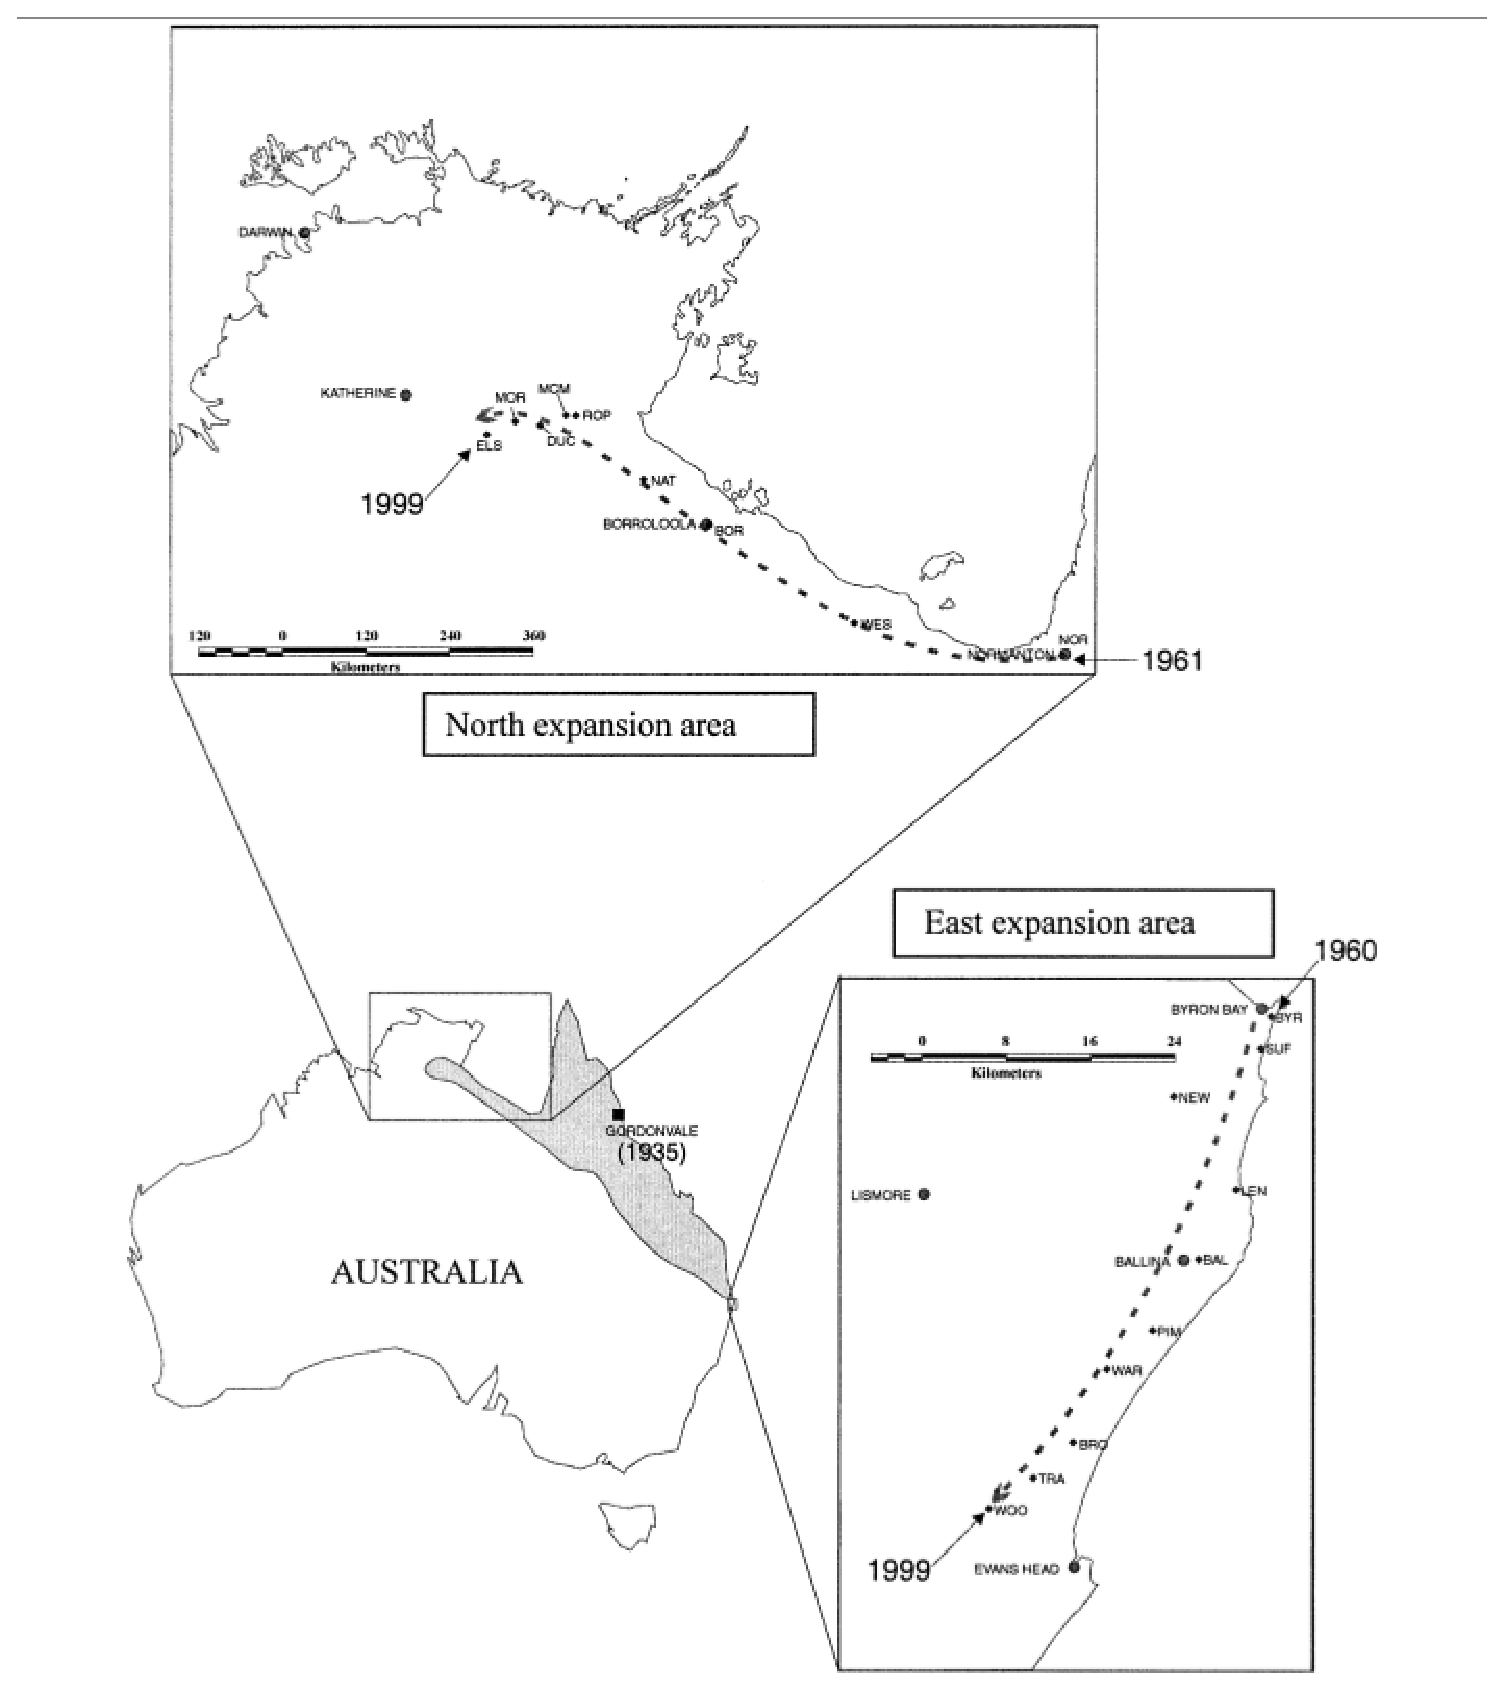
\includegraphics[height=\textheight]{cane-toad-expansion.eps}
\end{center}
}

\myslide{
\begin{center}
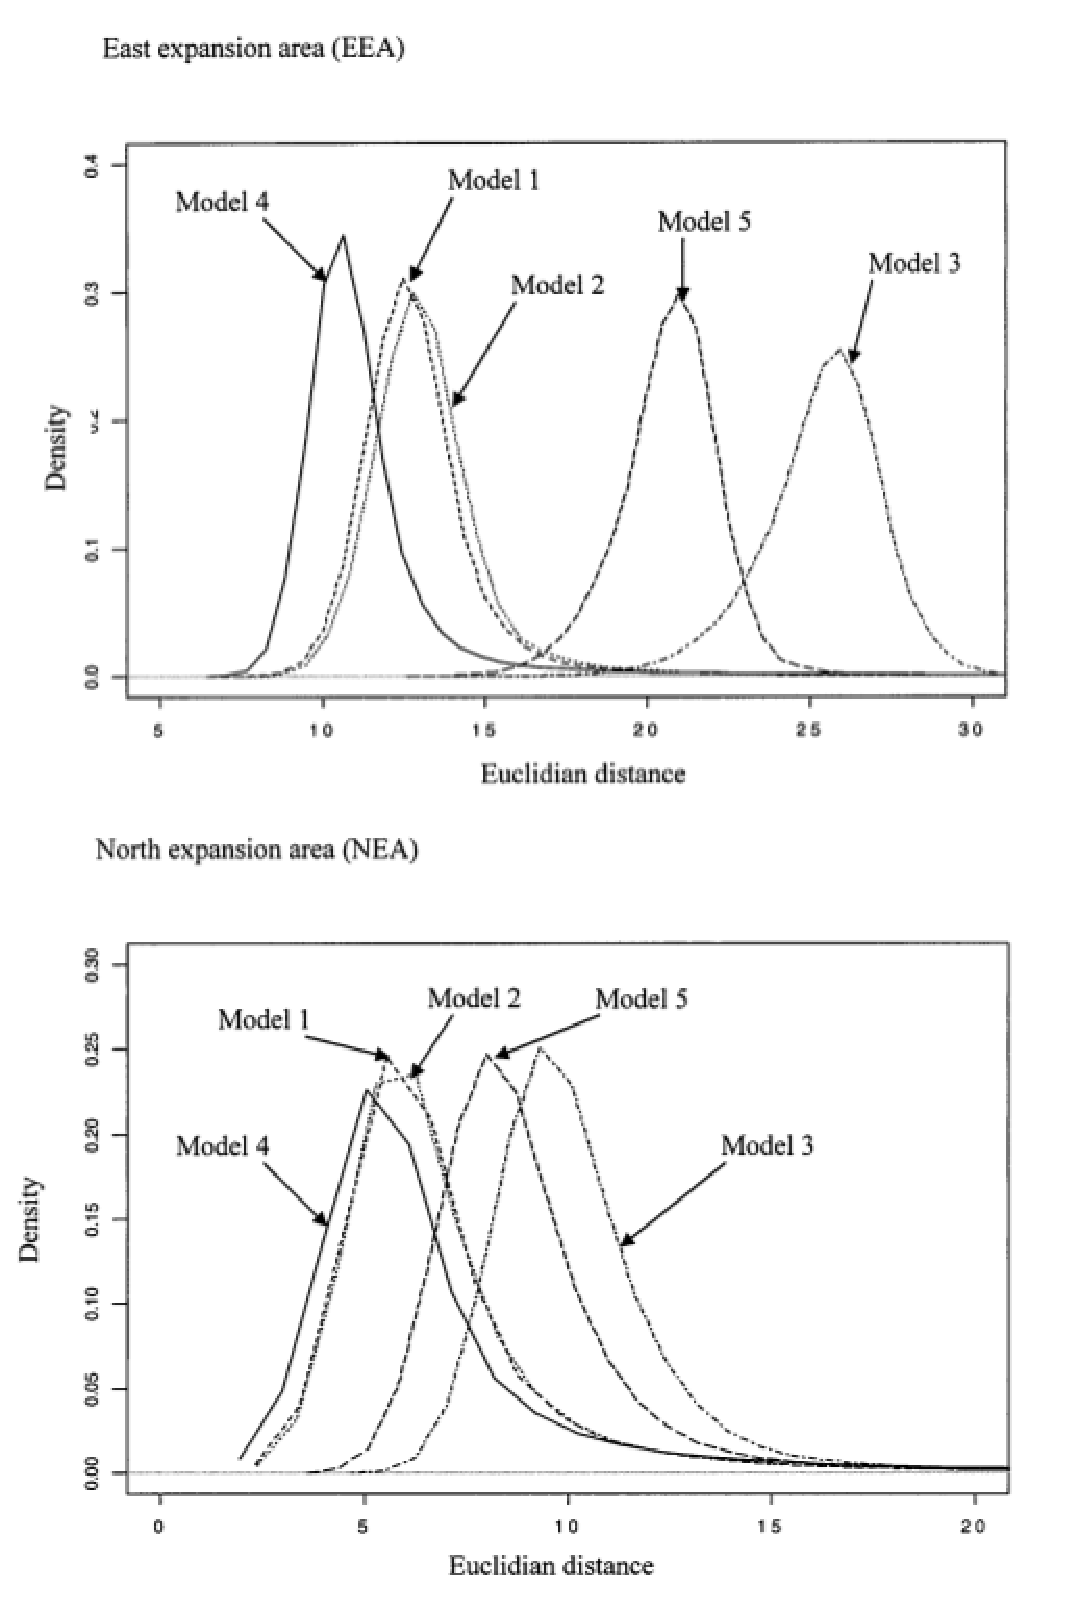
\includegraphics[height=\textheight]{cane-toad-models.eps}
\end{center}
}

\myslide{
\begin{center}
\begin{tabular}{ccr}
\hline\hline
Parameter & area & mean (5\%, 90\%) \\
\hline
$N_{e_s}$ & east & 744 (205, 1442) \\
         & north & 1685 (526, 2838) \\
$N_{e_f}$ & east & 78 (48, 118) \\
         & north & 311 (182, 448) \\
$F_R$    & east & 10.7 (2.4, 23.8) \\
         & north & 5.9 (1.6, 11.8) \\
$m$      & east & 0.014 ($6.0 \times 10^{-6}$, 0.064) \\
         & north & 0.117 ($1.4 \times 10^{-4}$, 0.664) \\
$N_{e_s}m$ & east & 4.7 (0.005, 19.9) \\
          & north & 188 (0.023, 883) \\
\hline
\end{tabular}
\end{center}
}

\myslide{
RAD sequencing

\begin{itemize}

\item Digest genomic DNA from each individual with a restriction
  enzyme, and ligate an adapter to the resulting fragments. The
  adapter includes a forward amplification primer, a sequencing primer
  and a ``barcode'' used to identify the individual from which the DNA
  was extracted.

\item Pool the individually barcoded samples~(``normalizing'' the
  mixture so that roughly equal amounts of DNA from each individual
  are present) shear them and select those of a size appropriate for
  the sequencing platform you are using.

\item Ligate a second adapter to the sample, where the second adapter
  is the reverse complement of the reverse amplification primer. 

\item PCR amplification will enrich only DNA fragments having both the
  forward and reverse amplification primer.

\end{itemize}

}

\myslide{
GBS

\begin{itemize}

\item Digest genomic DNA with a restriction enzyme and ligate two
  adapters to the genomic fragments. One adapter contains a barcode
  and the other does not.

\item Pool the samples.

\item PCR amplify and sequence. Not all ligated fragments will be
  sequenced because some will contain only one adapter and some
  fragments will be too long for the NGS platform.

\end{itemize}

}

\begin{center}
\includegraphics[height=0.9\textheight]{NGS-approaches.eps}
\end{center}

\begin{figure}
\begin{center}
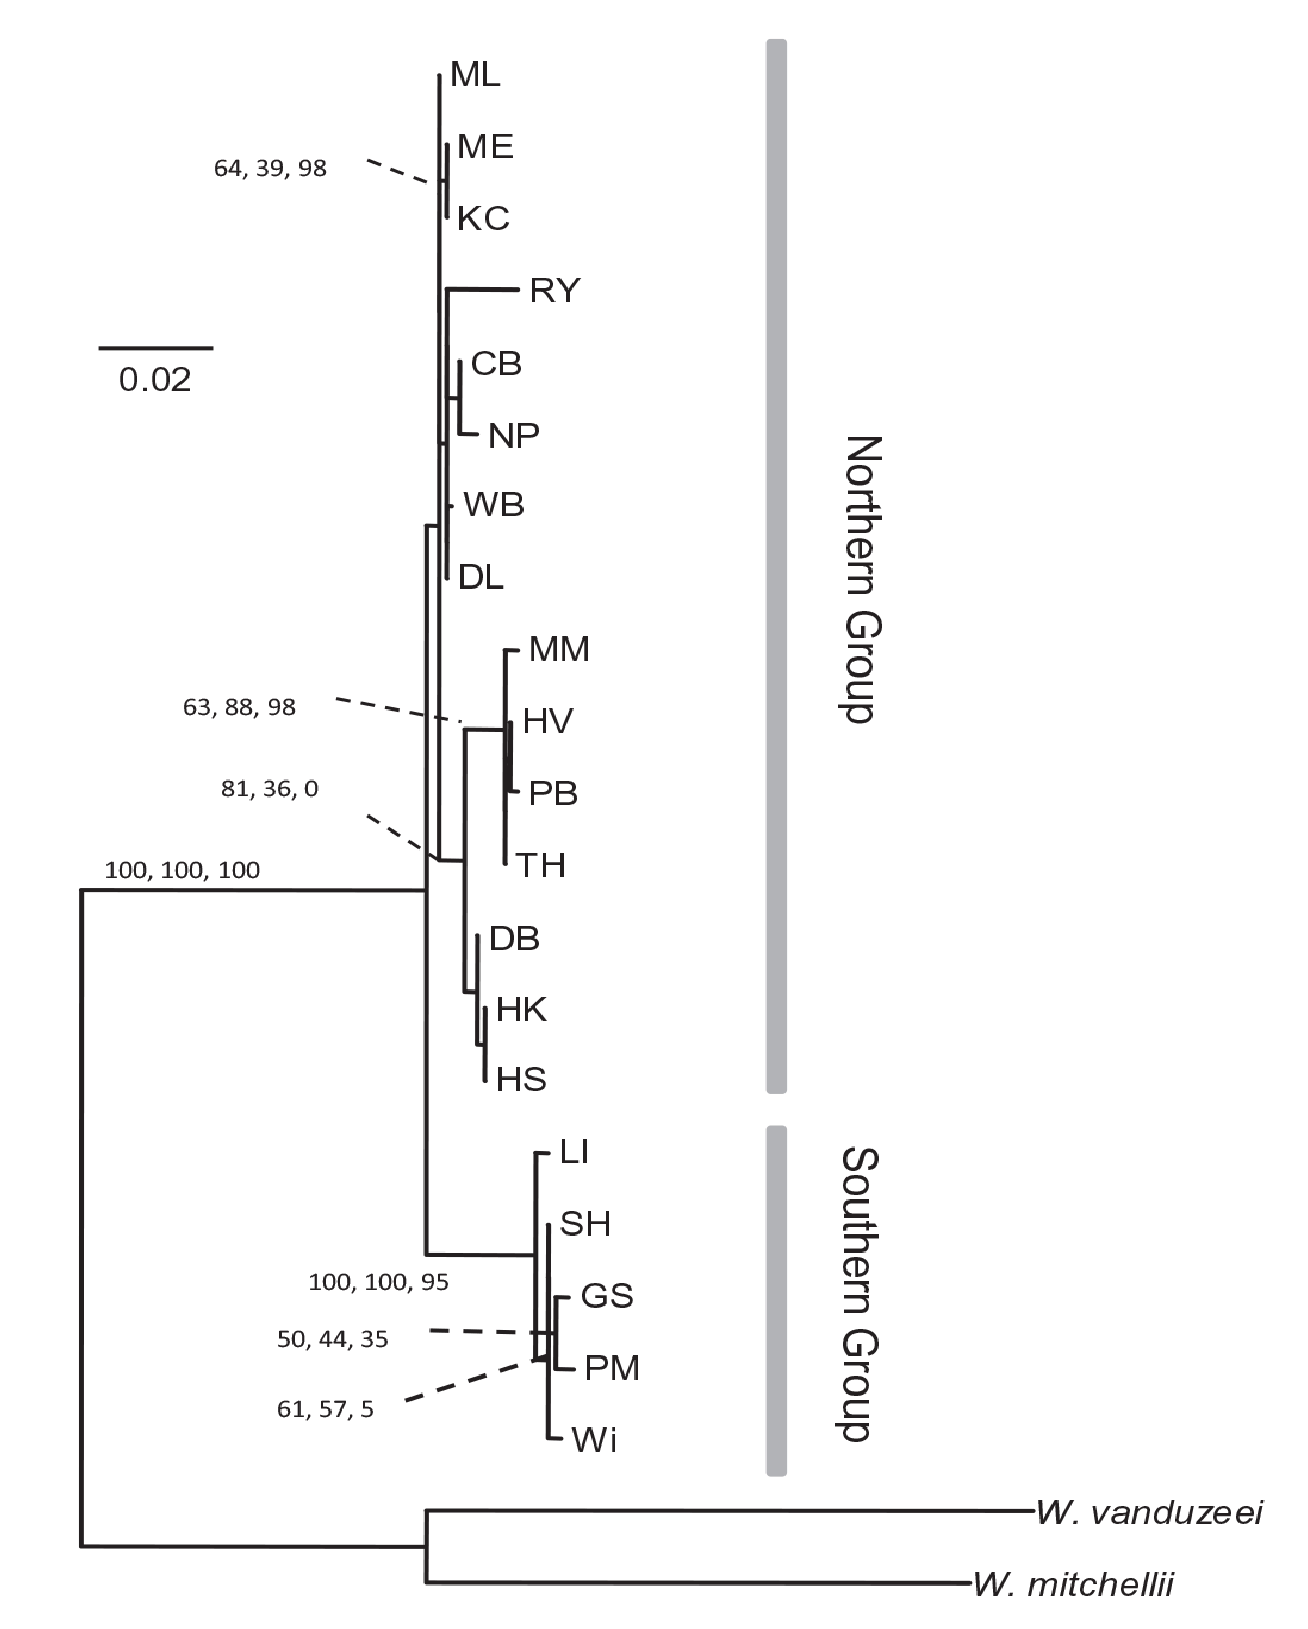
\includegraphics[height=0.8\textheight]{wyeomyia-COI.eps}
\end{center}
\caption{Maximum-likelihood phylogenetic tree depicting relationshps
  among populations of {\it W. smithii\/} relative to the outgroups
  {\it W. vanduzeei\/} and {\it W. mitchelli} based on analysis of
  {\it COI}.}
\end{figure}

\begin{figure}
\begin{center}
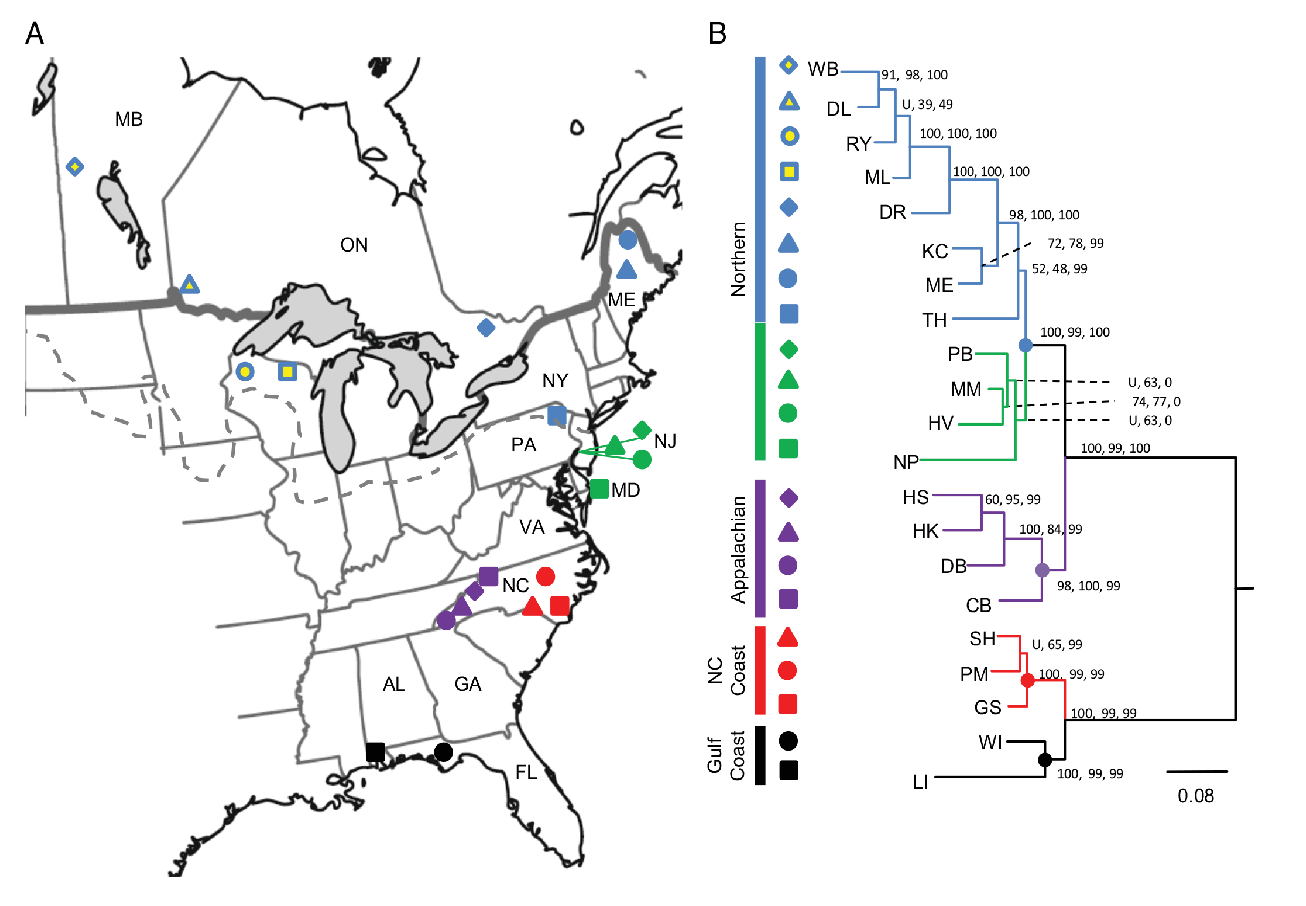
\includegraphics[height=0.8\textheight]{wyeomyia-RAD.eps}
\end{center}
\caption{Results from RAD sequencing (3741 SNPs) A. Geographical
  distribution of samples included in the analysis. B. Phylogenetic
  relationship of samples included in the analysis.}
\end{figure}

\myslide{
\begin{eqnarray*}
(n_1, n_2, n_3, n_4) &=& \mbox{no. of times A, C, G, T observed at a
  site} \\
\epsilon &=& \mbox{probability of sequencing error at a site} \\
\end{eqnarray*}
Suppose a particular site is really homozygous A. Our sequencing
should give us all A, but because of sequencing error, we might also
see some C, G, and T.
\begin{eqnarray*}
P(n_1,n_2,n_3,n_4|\mbox{homozygous A},\epsilon)
&=&
{n \choose n_1}(1-\epsilon)^{n_1}\epsilon^{n-n_1} \\
\end{eqnarray*}
}

\myslide{
\begin{eqnarray*}
(n_1, n_2, n_3, n_4) &=& \mbox{no. of times A, C, G, T observed at a
  site} \\
\epsilon &=& \mbox{probability of sequencing error at a site} \\
\end{eqnarray*}
Suppose a particular site is really homozygous A. Our sequencing
should give us all A, but because of sequencing error, we might also
see some C, G, and T.
\begin{eqnarray*}
P(n_1,n_2,n_3,n_4|\mbox{homozygous A},\epsilon)
&=&
{n \choose n_1}(1-\epsilon)^{n_1}\epsilon^{n-n_1} \\
P(n_1,n_2,n_3,n_4|\mbox{homozygous},\epsilon)
&=&
\sum_{i=1}^4 \left(\frac{p_i^2}{\sum_{j=1}^4p_j^2}\right) 
{n \choose n_i}(1-\epsilon)^{n_i}\epsilon^{n-n_i}
\end{eqnarray*}
}

\myslide{
\begin{eqnarray*}
k_1 &=& \mbox{number of reads from chromosome 1} \\
k_2 &=& \mbox{number of reads from chromosome 2} \\
n &=& k_1 + k_2 \\
P(k_1,k_2)
&=&
{n \choose k_1}\left(\frac{1}{2}\right)^{k_1}
               \left(\frac{1}{2}\right)^{k_2}
\\
&=&
{n \choose k_1}\left(\frac{1}{2}\right)^n
\end{eqnarray*}
}

\myslide{
{\tiny
\begin{eqnarray*}
P(n_1,n_2,n_3,n_4|x_i,x_j,k_1,k_2)
=
\sum_{l=1}^4\sum_{m=0}^{k_1}&&{k_1 \choose
  m}(1-\delta_{il})^m\delta_{il}^{k_1-m} \\
&\times&{k_2 \choose n-m}(1-\delta_{jl})^{n_1-m}\delta_{jl}^{k_2-(n_1-m)}
\end{eqnarray*}
}
\[
\delta_{il} = \left\{\begin{array}{ll}
1-\epsilon & \mbox{if } i = l \\
\epsilon & \mbox{if } i \ne l \quad .
\end{array}
\right.
\]
\[
P(n_1,n_2,n_3,n_4|x_i,x_j,\epsilon) =
P(n_1,n_2,n_3,n_4|x_i,x_j,k_1,k_2,\epsilon)P(k_1,k_2)
\]
{\footnotesize
\[
P(n_1,n_2,n_3,n_4|\mbox{heterozygous},\epsilon)
=
\sum_{i=1}^4\sum_{j\ne i}
\left(\frac{x_ix_j}{1-{\sum_{l=1}^4p_l^2}}\right) P(n_1,n_2,n_3,n_4|x_i,x_j) 
\]
}

}

\myslide{

\begin{eqnarray*}
P(n_1,n_2,n_3,n_4|\pi,\epsilon)
&=&
\pi P(n_1,n_2,n_3,n_4|\mbox{heterozygous},\epsilon) \\
&&+
(1-\pi)P(n_1,n_2,n_3,n_4|\mbox{homozygous},\epsilon) \\
P(\mbox{data}|\pi,\epsilon) &=& \prod_{s=1}^S
P(n_1^{(s)},n_2^{(s)},n_3^{(s)},n_4^{(s)}|\pi,\epsilon)
\end{eqnarray*}

}

\myslide{
\begin{center}
\begin{tabular}{lccc}
\hline\hline
Taxon & $4N_e\mu$ & $4N_e\mu$ (low coverage) & $\epsilon$ \\
\hline
{\it Cionia intestinalis} & 0.0111 & 0.012 & 0.00113 \\
{\it Daphnia pulex} & 0.0011 & 0.0012 & 0.00121 \\
\hline
\end{tabular}
\end{center}
}

\begin{center}
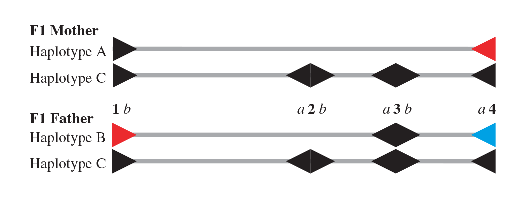
\includegraphics[width=0.9\textwidth]{RAD-heterozygosity.eps}
\end{center}

\begin{center}
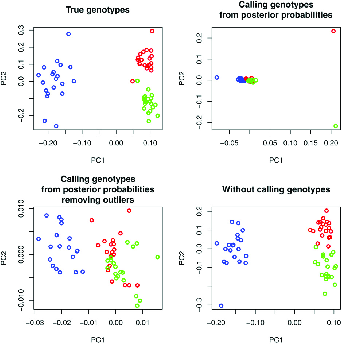
\includegraphics[width=0.8\textwidth]{fumagalli-PCA.eps}
\end{center}

\end{document}
